
\documentclass[a4paper,12pt,oneside]{article}

\usepackage[english]{babel}
\usepackage[utf8]{inputenc}
\usepackage[T1]{fontenc}
\usepackage{listings}
\usepackage{amsmath}
\usepackage{amsthm}
\usepackage{url}
\usepackage{verbatim}
\usepackage{graphicx}

\newtheorem{theorem}{Theorem}
\newtheorem{lemma}[theorem]{Lemma}

\title{Advanced Algorithms - Euclidean Travelling Salesman Problem}
\author{Samuel Wej\'eus \\ \lowercase{wejeus@kth.se} \and Peter Boström \\ \lowercase{pbos@kth.se} }

\begin{document}
\maketitle

\section{Introduction}
In the fields of computer science and mathematical optimization a well known problem is the \textit{tradelling salesman problem, or TSP}. The problem is often stated as follows: \textit{given a list of cities and their pairwise distances, find the shortest possible path that visit each city exactly once and then return to the start position}. It is easy to see how this can be transformed into a mathematical representation by using a graph. Each city is a node, let there be an edge from each city to every other city, each representing the distance between the two. The solution to the problem must then be an ordered subset of the edges with the constraints that two edges immediately following each other must end in a common vertex and there must be exactly $n$ vertices each occurring exactly once.

It is well know that the TSP is NP-complete and we will not dwell on details only mention that no deterministic algorithm\footnote{Deterministic used in the sense of reduction based problem structure, i.e. no guarantee in correctness of subproblems.} that finds an optimal solution currently exists, instead the most commonly used approach is to find some (possible bad) solution and then successively improve this solution until some halting criteria is met.

\section{Tour construction}
TODO

\section{Local optimization}
After arguing how to find the best possible starting tour we now look at how this tour can be improved further. Methods used typically builds on techniques to reconstruct the tour by making path changes. The more popular methods is \textit{2OPT, 3OPT} and \textit{Lin-Kernighan}. Starting with the foremost, in 2OPT we try to find a better tour by successively testing if an exchange of two edges at a time would result in an improvement of tour cost, if so perform the exchange and continue with an other two pair of nodes.

Regarding 3OPT and Lin-Kernighan, or LK for short, both can be seen as extensions of 2OPT - building on the same idea of edge exchange where in 3OPT you test three edges at a time and LK can be seen as a generalization to $n$ edge exchanges at a time.

The variation in how many edges are exchanged at one time gives the various techniques different characteristics, namely difference in running time and cost of total tour found. The difference in tour cost is obviously expected since they are all \textit{local} optimization techniques and no guarantee exists that any local improvement actually is a part of any global \textit{optimal} solution (side note: this is what we refer to by \textit{non-determenistic} in the introduction, see footnote 1).

All three local optimization procedures given above have different aspects and properties that make the unique. From results given in \cite{localopt} we see that a higher running, on average, normally produces a better tour cost. As an example taken from \cite{localopt}, the difference in running time between LK and 2OPT on an input size of $10^6$ is 2650 vs 940 seconds and the average excess over Held-Karp lower bound is 2.0 vs 4.9 in favor of LK. But if running time is of more importance the higher tour cost might be acceptable. This shows that there is no clear definition of \textit{"best"} approach for local optimization instead its up to the needs of the context. 

%% is this correct? =)
Most important to us we deemed to be time. This due to how the judging is structured on \textit{Kattis}. We sacrifice some improvement in tour cost to instead be able to run more test and in that way (hopefully) score more points. Our final choice was 2OPT.



\subsection{Reversing edges}
Using 2OPT algorithm we note that when two edges are exchanged (i.e a new connection between \textit{four} independent nodes is established) no matter how we create these new edges the result of the exchange will \textit{never} form a directed cycle. This is due to the fact that regardless of which edge we exchange for (and independently of direction) the result will always be exactly one node will have two edges directed towards it and exactly one node with two exiting edges, no other assignment is possible. See figure below for illustration, note the directions of edges.

\begin{figure}[h]
	\begin{center}
		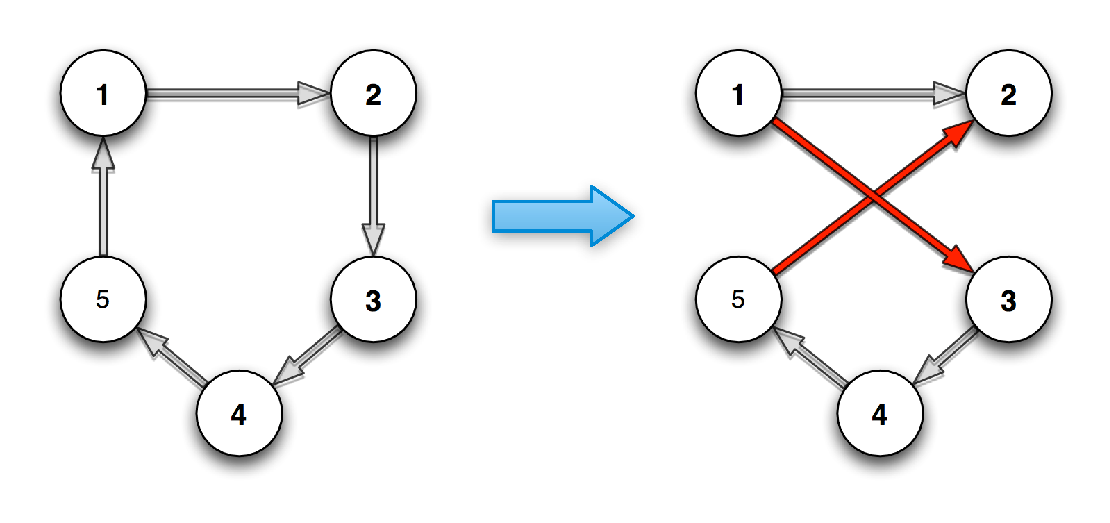
\includegraphics[width=0.90\linewidth]{rev_edge_graph.eps}
	\end{center}
	\caption{Exchanging edges}
	\label{exchange}
\end{figure}


Looking at the graph this way we it is clear that we can divide it into two disjoint sets with the exchanged edges being the interconnection between the two. Since each half in itself is correctly directed to create a new directed graph of the union of the disjoint sets only one of the two sets needs to be reversed. A local optimization we investigated was if we where able to determine or at least approximate the size of each set we could make reversing edges more efficient by choosing the smaller set. 

To calculate the size of any of the sets we must be able to determine its size for any node since the edges picked for exchange can be picked arbitrarily. This means the the only way to determine the size of the set is to traverse set linearly starting and stopping in any of the two nodes involved in the edge exchange. If we denote the size of a graph as $|N|$ and the size of the two disjoint sets as $|A|$ resp. $|B|$ we then know that $|B| = |N| - |A|$ this means that if we, while calculating the size for $A$, come to a point where $|A| > \frac{|N|}{2}$ we can conclude that $B$ is smaller and then reverse the edges of the set $B$. The problem with this approach is that if we while investigating the size of a set conclude that the \textit{other} set is smaller and reverse that set the result would be that we have visited $|N|$ nodes in total which is not desired. 

The argument above also shows that no other approximation is possible and we further believe that the use of additional data structures to keep track of set size for various nodes is not possible due the fact that edges can be exchange at random as shown above.

In our implementation we simply pick the set arbitrarily and reverse the edges of that set. Since the edges involved in the 2OPT exchange is picked at random and we pick one set out of two who's union forms the entire graph we state, without proof that the average size of the set picked will have have a size of $\frac{1}{2} \times |N|$.


%Further things to note: pick node with 2 inclining edges, traverse until ingen utfallande edge finns = KLART med get settet behover nu bars reverse kant inblandad i exchange

\begin{thebibliography}{9}

\bibitem{localopt}
	D. Johnson and L. McGeoch,
	\emph{The Traveling Salesman Problem: A Case Study in Local Optimization. in Local Search in Combinatorial Optimization}.
	E. H. L. Aarts and J. K. Lenstra (eds), John Wiley and Sons, Ltd., 1997, pp. 215-310. http://www2.research.att.com/~dsj/papers.html

\end{thebibliography}

\end{document}


